\chapter{Introduction}\label{sec:introduction}
[@bugwelle Introduction(1/2)]

\section{Common Fundamentals}\label{sec:introduction_common_fundamentals}
All articles build upon a common set of fundamental definitions regarding software testing and requirements.
They are listed and mapped to the individual topics in the glossary section of this report.
It is highly recommended to refer to the glossary before reading an article or when ambiguities arise while reading an article.
However, since it is quite extensive and also contains more topic-specific definitions, the most important terms are defined hereafter.

Like a part of the entries in the glossary section, we use the \enquote{Guide to the Software Engineering Body of Knowledge} (short: SWEBOK) in its third version as a basis.
Although this guide is already quite old (at least the original version from 2004), hence not fully compliant with current research results, its 15 knowledge areas and basic definitions of a body of knowledge are still useful for classifying the approaches presented in this report and establish a common set of technical terms.

Let us begin with requirements.
The corresponding SWEBOK knowledge area is \enquote{Software Requirements}.
Relevant sub chapters are \enquote{Software Requirements Fundamentals} and \enquote{Requirements Validation}.
The guide defines requirements as \enquote{a property that must be exhibited by something in order to solve some problem in the real world. [\ldots]
An essential property of all software requirements is that they be verifiable as an individual feature as a functional requirement or at the system level as a non-functional requirement.
It may be difficult or costly to verify certain software requirements.} \cite{SWEBOK}
This definition already points out the difficulty of verifying requirements that necessitates the use of systematic testing techniques, as explained in \autoref{sec:introduction_common_fundamentals}.
Moreover, it distinguishes between functional, representing a feature the software is to provide, and non-functional requirements, specifying the extend of quality.
Requirements need to be formulated clearly, unambiguously and quantitatively in order to implement and verify them correctly \cite{SWEBOK}.

For software testing, there is no uniform definition.
Therefore, the guide refers to multiple definitions from cited references.
In essence, software testing is to assure that specified requirements are met by the implementation or, from a different perspective, find errors indicating that a requirement has not been met.
This testing process is performed at different levels, as the requirements definition already touched upon. % ???
The SWEBOK guide distinguishes between three test levels: unit testing, verifying isolated functionalities (mostly functional requirements), integration testing, verifying the correct interaction of components and system testing, verifying the behavior of the entire system (mostly non-functional requirements).
Correspondingly, these levels are distinguished by the object of the test (single module, multiple modules, entire system), called the target of the test, and the purpose, called objective of the test \cite{SWEBOK}.

The guide presents a wide array of testing techniques.
For this report, it is important to take notice of the definition of model-based testing: \enquote{A model in this context is an abstract (formal) representation of the software under test or of its software requirements (see Modeling in the Software Engineering Models and Methods KA).
Model-based testing is used to validate requirements, check their consistency, and generate test cases focused on the behavioral aspects of the software.}\cite{SWEBOK}
Some of the approaches presented in this report are model based, at least partially.
However, it is not always clear what the actual model is and some authors use the term incorrectly.

Finally, it is important to emphasize the difference between different artifacts produced during the testing process, including the afore-mentioned test objectives, test cases (logical or concrete with inputs) as well as executable tests (as code).

\section{Outline}

Following this introduction in \autoref{sec:introduction}, nine individual reports each present two different but related approaches for systematic testing in Sections 2\,-\,10.
The reports introduce their superordinate topic in Sections X.1, outline the results and execution of a literature search based on a given article in Sections X.2 and describe the given and selected approach in Sections X.3.1 and X.4.1 as well as illustrating them using a common set of given requirements in Sections X.3.2 and X.4.2.
Finally, the approaches are compared using a common set of questions in Sections X.5 and evaluated in Sections X.6.
Section 11 concludes the report.
The glossary and bibliography can be found in Sections 12 and 13.
In the following, the given requirements (\autoref{fig:mm}) and synthesis questions, used for each individual report, are depicted.

\textbf{Synthesis questions:}

\begin{enumerate}
	\item What is the name of the approach? If no name is provided, the publication title is used.
	\item Summary
	\item Description of the approach (What does the approach do?)
	\begin{enumerate}
		\item Which artifacts and relations between artifacts are used in this approach? Which artifacts are created in the course of the approach? How are the artifacts characterized?
		\item What is required and/or input for the application of the approach?
		\item What steps does the approach consist of? Which information is used in which step and how? What are the results of the individual steps?
	\end{enumerate}
	\item Benefits of the approach (Whom does the approach help and how?)
	\begin{enumerate}
		\item Which usage scenarios are supported by the approach?
		\item Which stakeholders are supported by the usage scenarios?
		\item Which knowledge areas from SWEBOK can be assigned to the usage scenarios?
	\end{enumerate}
	\item Tool support for the approach (What tool support is available?)
	\begin{enumerate}
		\item What tool support is provided for the approach?
		\item Which steps of the approach are automated by a tool? Which steps are supported by a tool, but still have to be executed manually? Which steps are not supported by a tool?
	\end{enumerate}
	\item Quality of the approach (How well does the approach work?)
	\begin{enumerate}
		\item How was the approach evaluated?
		\item What are the (main) results of the evaluation?
	\end{enumerate}
\end{enumerate}

\newpage
\newgeometry{margin=1cm}
\begin{landscape}

\begin{figure}
	\centering
	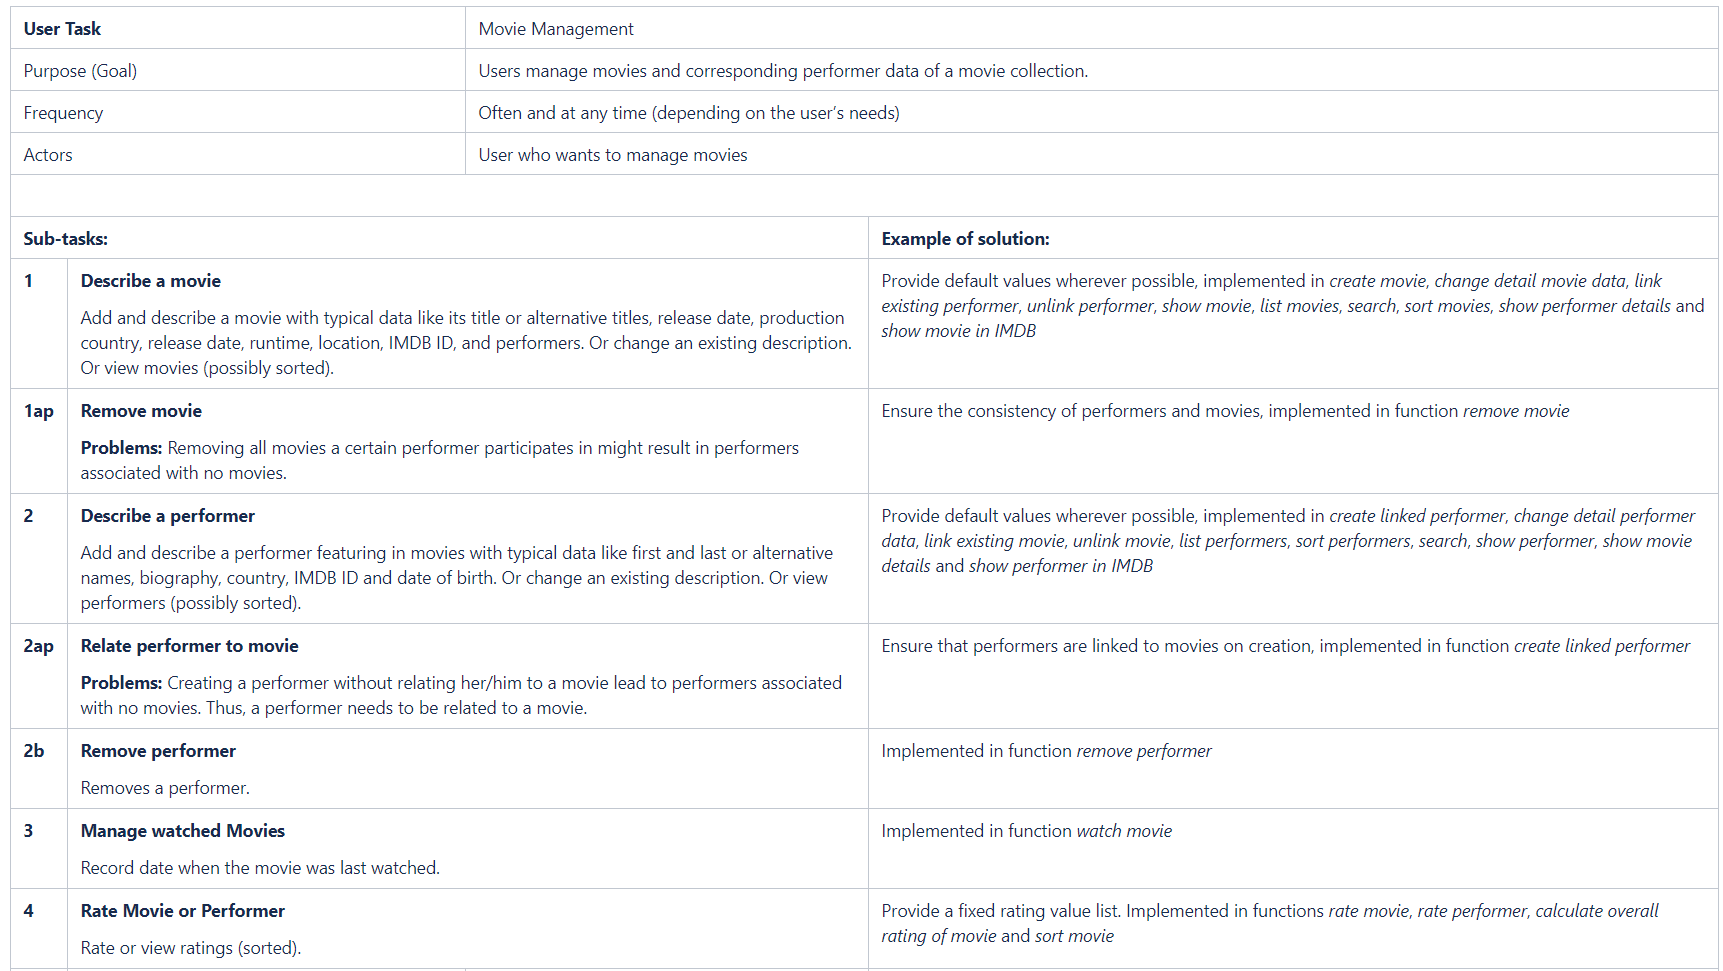
\includegraphics[scale=0.57]{../images/MovieManager.png} 
	\caption{Requirements in User-Task notation for the MovieManager software, a mobile application for managing movie collections.}
	\label{fig:mm}
\end{figure}

\end{landscape}
\restoregeometry


